\documentclass[conference]{IEEEtran}

\usepackage{graphicx} % For including images
\usepackage{amsmath} % For mathematical symbols and equations
\usepackage{hyperref} % For hyperlinks
\usepackage{caption}
\usepackage{amsfonts} % For math fonts and symbols
\usepackage{booktabs} % For better tables
\usepackage{listings} % For code listings
\usepackage{multirow} % For multi-row cells in tables

\begin{document}
	
	\title{Data Management \\ Project of a Data Warehouse System for Analyzing Meteorite Landings by NASA}
	
	\author{
		\IEEEauthorblockN{Giuseppe Valente - Natalia Maria Mucha}
		\IEEEauthorblockA{
			Engineering in Computer Science \\
			Sapienza University of Rome \\
		}
	}
	\maketitle
	
	\begin{abstract}
			This project focuses on developing a data warehouse system to integrate and analyze meteorite landing data from NASA. The objective is to demonstrate how to design and implement a data warehouse on a relational database using ETL processes, a dimensional fact model (DFM) schema, and Postgres SQL for deployment. 
	\end{abstract}
	
	\section{Introduction}
	
	This project aims to develop a data warehouse system specifically designed to integrate and analyze data on meteorite landings using NASA's Meteorite Landings dataset. The project’s objective is to demonstrate how to design and implement a data warehouse on a relational database platform using Postgres SQL. The process involves the application of Extract, Transform, Load (ETL) techniques to systematically collect, clean, and organize the data. Additionally, the project employs a Dimensional Fact Model (DFM) schema to structure the data in a way that supports in-depth analysis. \\ The result is a powerful tool for advancing the study of meteorites and their impacts on Earth.
	
	\section{Data warehouse}
	A data warehouse (DWH), is a system used for reporting and data analysis, are central repositories of integrated data from one or more sources. They store current and historical data in one single place that are used for creating reports. This is beneficial for companies as it enables them to interrogate and draw insights from their data and make decisions.

	\section{Datasets}
	
	\subsection{Meteorite Landings Dataset}
	This comprehensive data set from The Meteoritical Society contains information on all of the known meteorite landings. The Fusion Table is collected by Javier de la Torre and we've also provided an XLS file that consists of 34,513 meteorites. \\
	\href{https://data.nasa.gov/Space-Science/Meteorite-Landings/gh4g-9sfh/about_data}{NASA's Open Data Portal}
	
	\subsection{Meteoritical Bulletin Database}
	This database has been constructed and is maintained by the Nomenclature Committee of the Meteoritical Society. The primary function of this database is to provide authoritative information about meteorite names. The correct spelling, complete with punctuation and diacritical marks, of all known meteorites recognized by the Meteoritical Society may be found in this compilation. Official abbreviations for many meteorites are documented here as well. The database also contains status information for meteorites with provisional names, and listings for specimens of doubtful origin and pseudometeorites. \\
	\href{https://www.lpi.usra.edu/meteor/}{Lunar and Planetary Institute}
	
	\subsection{Socrata Location}
	Dataset used to revert the coordinate point from latitude,longitude to human readable format.
	\href{https://dev.socrata.com/docs/datatypes/location.html#}{Tyler Technologies - Socdata}
	
	\section{System Architecture}
	The first techincal choise is the system architecture to realize, typically between the two-layer and three-layer architecture, for this reason we have a brief of the how the two architectures are composed:
	
	\subsection{Two-Layer Architecture (2LA)}
	\begin{figure}[h]
		\centering
		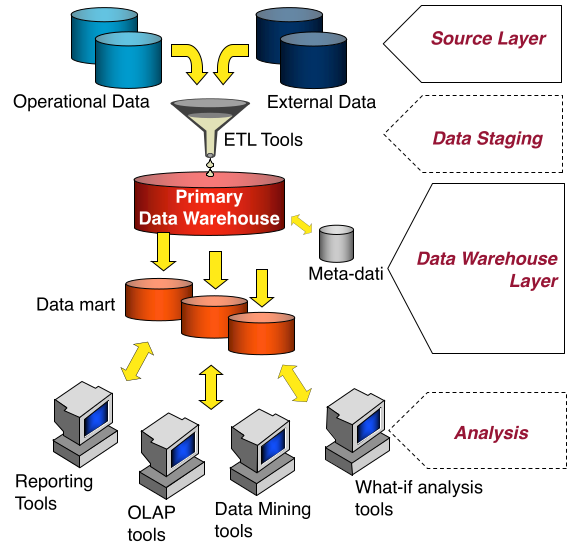
\includegraphics[width=\columnwidth]{images/two_layer_architecture.png}
		\caption{Two Layer Architecture}
		\label{fig:two layer architecture}
	\end{figure}
	The 2LA is an architecture composed by two mainly elements, the sources and the DWH.
	In this architecture the data marts (a simple form of a DWH that is focused on a single subject, hence they draw data from a limited number of sources such as sales, finance or marketing) from an architectural point of view are considerated as the presentation layer of the architecture.
	This architecture is very useful in organization from mid to large size and has the folowing advantages:
	\begin{itemize}[leftmargin=1cm]
		\item \textbf{Reliable Data Access:} DWH ensure that high-quality information is consistently available, even if the source systems are temporarily inaccessible due to technical or organizational issues.
		
		\item \textbf{Uninterrupted Operations:} Analytical queries in a DWH don't interfere with the daily transactional processes, which are critical for the smooth functioning of an organization's operations.
		
		\item \textbf{Structured for Analysis:} DWH are organized using a multidimensional model, which is more suitable for analysis, unlike the relational or semi-structured models typically used in operational systems.
		
		\item \textbf{Time and Granularity Differences:} DWH manage historical and summarized data for analysis, unlike OLTP systems that handle current, highly detailed data, highlighting a difference in time and data granularity.
		
		\item \textbf{Optimized for Performance:} DWH are designed with specific features to enhance the performance of analysis and reporting, ensuring faster and more efficient data processing.
	\end{itemize}
	
	
	\subsection{Three-Layer Architecture}
	\begin{figure}[h]
		\centering
		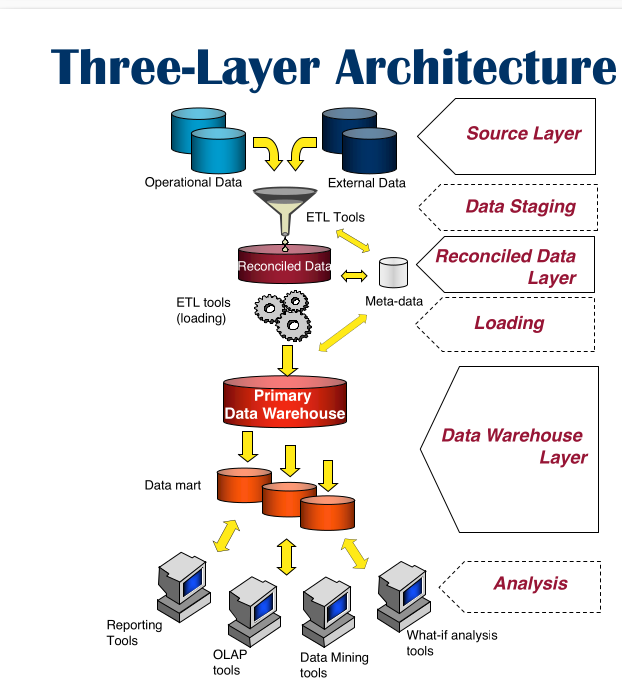
\includegraphics[width=\columnwidth]{images/three_layer_architecture.png}
		\caption{Three Layer Architecture}
		\label{fig:two layer architecture}
	\end{figure}
	
	
	\subsection{Overview}
	The data warehouse system is designed to integrate, store, and analyze data from the selected datasets. The system architecture includes the following components:
	
	\begin{itemize}
		\item \textbf{Data Extraction:} Data is extracted from NASA, IGNV, and GDIS sources.
		\item \textbf{Data Transformation:} Geocoding and data cleaning processes are applied to standardize the data formats.
		\item \textbf{Data Loading:} The cleaned data is loaded into a relational database system such as MySQL or PostgreSQL.
		\item \textbf{Data Analysis:} SQL queries and data visualization techniques are used to uncover patterns and correlations.
	\end{itemize}
		
	\section{ETL Process}
	
	\subsection{Extract}
	Data extraction scripts are written in Python, using libraries like `pandas` to read and process data files.
	
	\subsection{Transform}
	The transformation process includes converting geo-coordinates to human-readable formats and normalizing data formats across all datasets.
	
	\subsection{Load}
	The transformed data is loaded into the relational database using SQLAlchemy in Python, ensuring that all datasets are correctly integrated for analysis.
	
	\section{Dimensions Fact Model (DFM)}
	
	\section{Relational Database realization}

	\section{Conclusion}
	
	\section{Reference}
	
	
	
	
	
\end{document}
